\documentclass[aps,prl,10pt,twocolumn,floatfix]{revtex4-2}
\usepackage{graphicx}
\usepackage{dcolumn}
\newcolumntype{d}{D{.}{.}{-1}}
\usepackage{url}
\usepackage{physics}

\bibliographystyle{apsrev4-2}


\begin{document}

\begin{abstract}
A rotating mirror is a device that, when supplied a certain voltage, will rotate a mirror inside a cavity at a certain rotational frequency. 
If a laser is shot into this cavity and reflected off the rotating mirror to another mirror, and shot back at the cavity, the rotating mirror will have rotated some extra amount between the first and second impact.
If the rotational velocity of the mirror, the distance between the mirror, laser, and rotating mirror, and change in angle is known, someone can calculate the speed of light!
If our experiment we found the speed of light to be $2.987(35)\times 10^{8}m/s^2$, which is within $2\sigma$ of the known value of the speed of light, $299792458m/s^2$.
\end{abstract}


\title{Measuring the Speed of Light Using a Rotating Mirror}
\author{C. T. Rochelle}
\email{ctr233@msstate.edu}
\author{K. J. Grimes}
\date{\today}
\affiliation{Department of Physics and Astronomy\\Mississippi State University\\Mississippi State, MS 39762-5167}
\date{\today}

\maketitle

\section{Introduction}\label{Intro}
% Lead Up to Creation
Of all the universal constants, one of the most important, if not the most important, is the speed of light!
As we know now, $299792458m/s^2$, the current accepted value of the speed of light in a vacuum, is the fastest speed that any object can travel!
This value is of utmost important in all fields of physics, especially electromagnetism and relativity.
The speed of light is so important that scientists defined it to a value and defined what a meter is by a specified fraction of this known quantity!
The length of everything is relative to the speed of light.
How did we come to know this value?

Some of the earliest scientific work into the speed of light was done by Galileo \cite{light}!
He and his assistant stood on hilltops far away from each other and one of them held a lamp with a shade \cite{light}.
On queue, the person with the lamp would open the shade and the other person would mark down when they saw the light \cite{light}. 
From this experiment Galileo concluded that the speed of light was ``if not instantaneous, it is extraordinarily rapid" \cite{engineer}.

Knowing whether the speed of light was instant or very fast remained a mystery to physicists until the work of Ole Christensen Romer,  half a century after Galileo's work \cite{light}. 
He was a Danish astronomer who was studying the eclipse patterns of Jupiter and its moons \cite{light}.
From his data Romer tried to make predictions on when eclipses on Jupiter' by its moons would occur;
however, there was an inconsistency in his data and his observations. 
The times of the eclipses would ebb and flow with the months and orbits of the planets.
He factored this information into his charts and calculations and began to correctly predict the time of the eclipses!
He explained this by saying the distances between Jupiter and his moons and the Earth would vary by orbit location, and that the time delay factored into his equations was the speed of light!
He was unable to get an estimate on the orbit radius of Jupiter or the Earth so he could not calculate this value, but he did prove that light was not instantaneous \cite{light}!

If we fast forward 200 years to the 1850s, we see not much new information since the time of Romer;
however this changed with two similar inventions by two men, Armand Fizeau and Jean Foucault \cite{light}. 
Fizeau created a spinning wheel with teeth that light could pass through. 
His idea was that if you created a wheel with teeth spaced precisely enough, you could let the light pass through on the tooth slits, reflect off the back wall, and pass through the slits again \cite{light}!
This would only work if the teeth were at certain distances.
Jean Foucault, instead of using a lot of wheels with differently spaced teeth, used a rotating mirror instead.
His experiment relied on a laser being shot into a rotating mirror, fired off and then hitting the rotating mirror again!
Between the first and second impact of the photon on the rotating mirror, the mirror will have rotated some extra distance.
He measured that distance using a detection plate and calculated the speed of light from that!
Foucault's work is what this experiment is based on.

\section{Theory}\label{Theory}
% Derivation of Formula 
The most basic form of the equation for the speed of any object is 
\begin{equation}\label{base}
v=\frac{d}{t	}.
\end{equation}
This equation works for any object traveling at a fixed velocity. 
Light satisfies this condition, so we can use Equation \ref{base}, plugging in $c$, the speed of light, into velocity and $2D$, where $D$ is the distance from the rotating mirror and the final mirror, into $d$, giving
\begin{equation}\label{plug}
c=\frac{2D}{t}
\end{equation}
where $t$ is the time it takes light to travel the specified distance. 

Time, $t$, is the only unknown variable left, and we can find it from looking closer at the physics of the rotating mirror.
For each voltage value the rotating mirror rotated at a constant angular velocity, $\omega$, given by 
\begin{equation}\label{omega}
\omega=\frac{\delta \theta}{t}.
\end{equation}
We know from the law of reflection that 
\begin{equation}
\theta_i = \theta_r
\end{equation}
where $\theta_i$ is the incident angle and $\theta_r$ is the reflected angle. 
From this we can see that the angle of the reflected light will be $2\theta_i$ for a stationary mirror;
however, we are using a rotating mirror, not a stationary one!
Therefore, the mirror would have turned some extra rotation between $\theta_i$ and $\theta_r$, called $\delta \theta$.
So for a rotating mirror, the path angle will be twice the rotating angle by the law of reflection, giving $2\theta_i + 2\delta \theta$. 
If we look at the geometry of this system by looking at Figure \ref{schematic}, we see that the some $\delta \theta$ in the rotating mirror at point B, will cause some deviation, $\delta x$, of the laser dot on the detector at point W after traveling distance BQW, which I will refer to as $d$.
We can now relate these three values using a geometrical function
\begin{equation}\label{tan}
\tan{2\delta \theta}=\frac{\delta x}{d}.
\end{equation}
One approximation we can make at this step is the small angle approximation because $\delta \theta$ will be very close to zero because we make the assumption that $c \gg \omega$, meaning that we can simplify Equation \ref{tan} to
\begin{equation}\label{fintheta}
2\delta \theta=\frac{\delta x}{d}.
\end{equation}

We can now reorganize Equation \ref{fintheta} to solve for $\delta \theta$ and Equation \ref{omega} to solve for $t$ and plug in to the Equation \ref{plug} to get 
\begin{equation}
c=\frac{4dD\omega}{\delta x}.
\end{equation}
One important thing to notice is that $d$ and $D$ are actually equal to each other due to the setup of the problem!
If we look at Figure \ref{schematic}, we see that WQBC is equal to CD;
therefore $d=D=l$.
Since we did not measure $\omega$ directly, I will make the substitution to frequency with the conversion of $\omega=2\pi f$ to obtain an equation that is in the form of all known variables
\begin{equation}\label{answer}
c=\frac{8\pi l^2f}{\delta x}.
\end{equation}

\section{Experiment}
% What did you do?

\begin{figure}
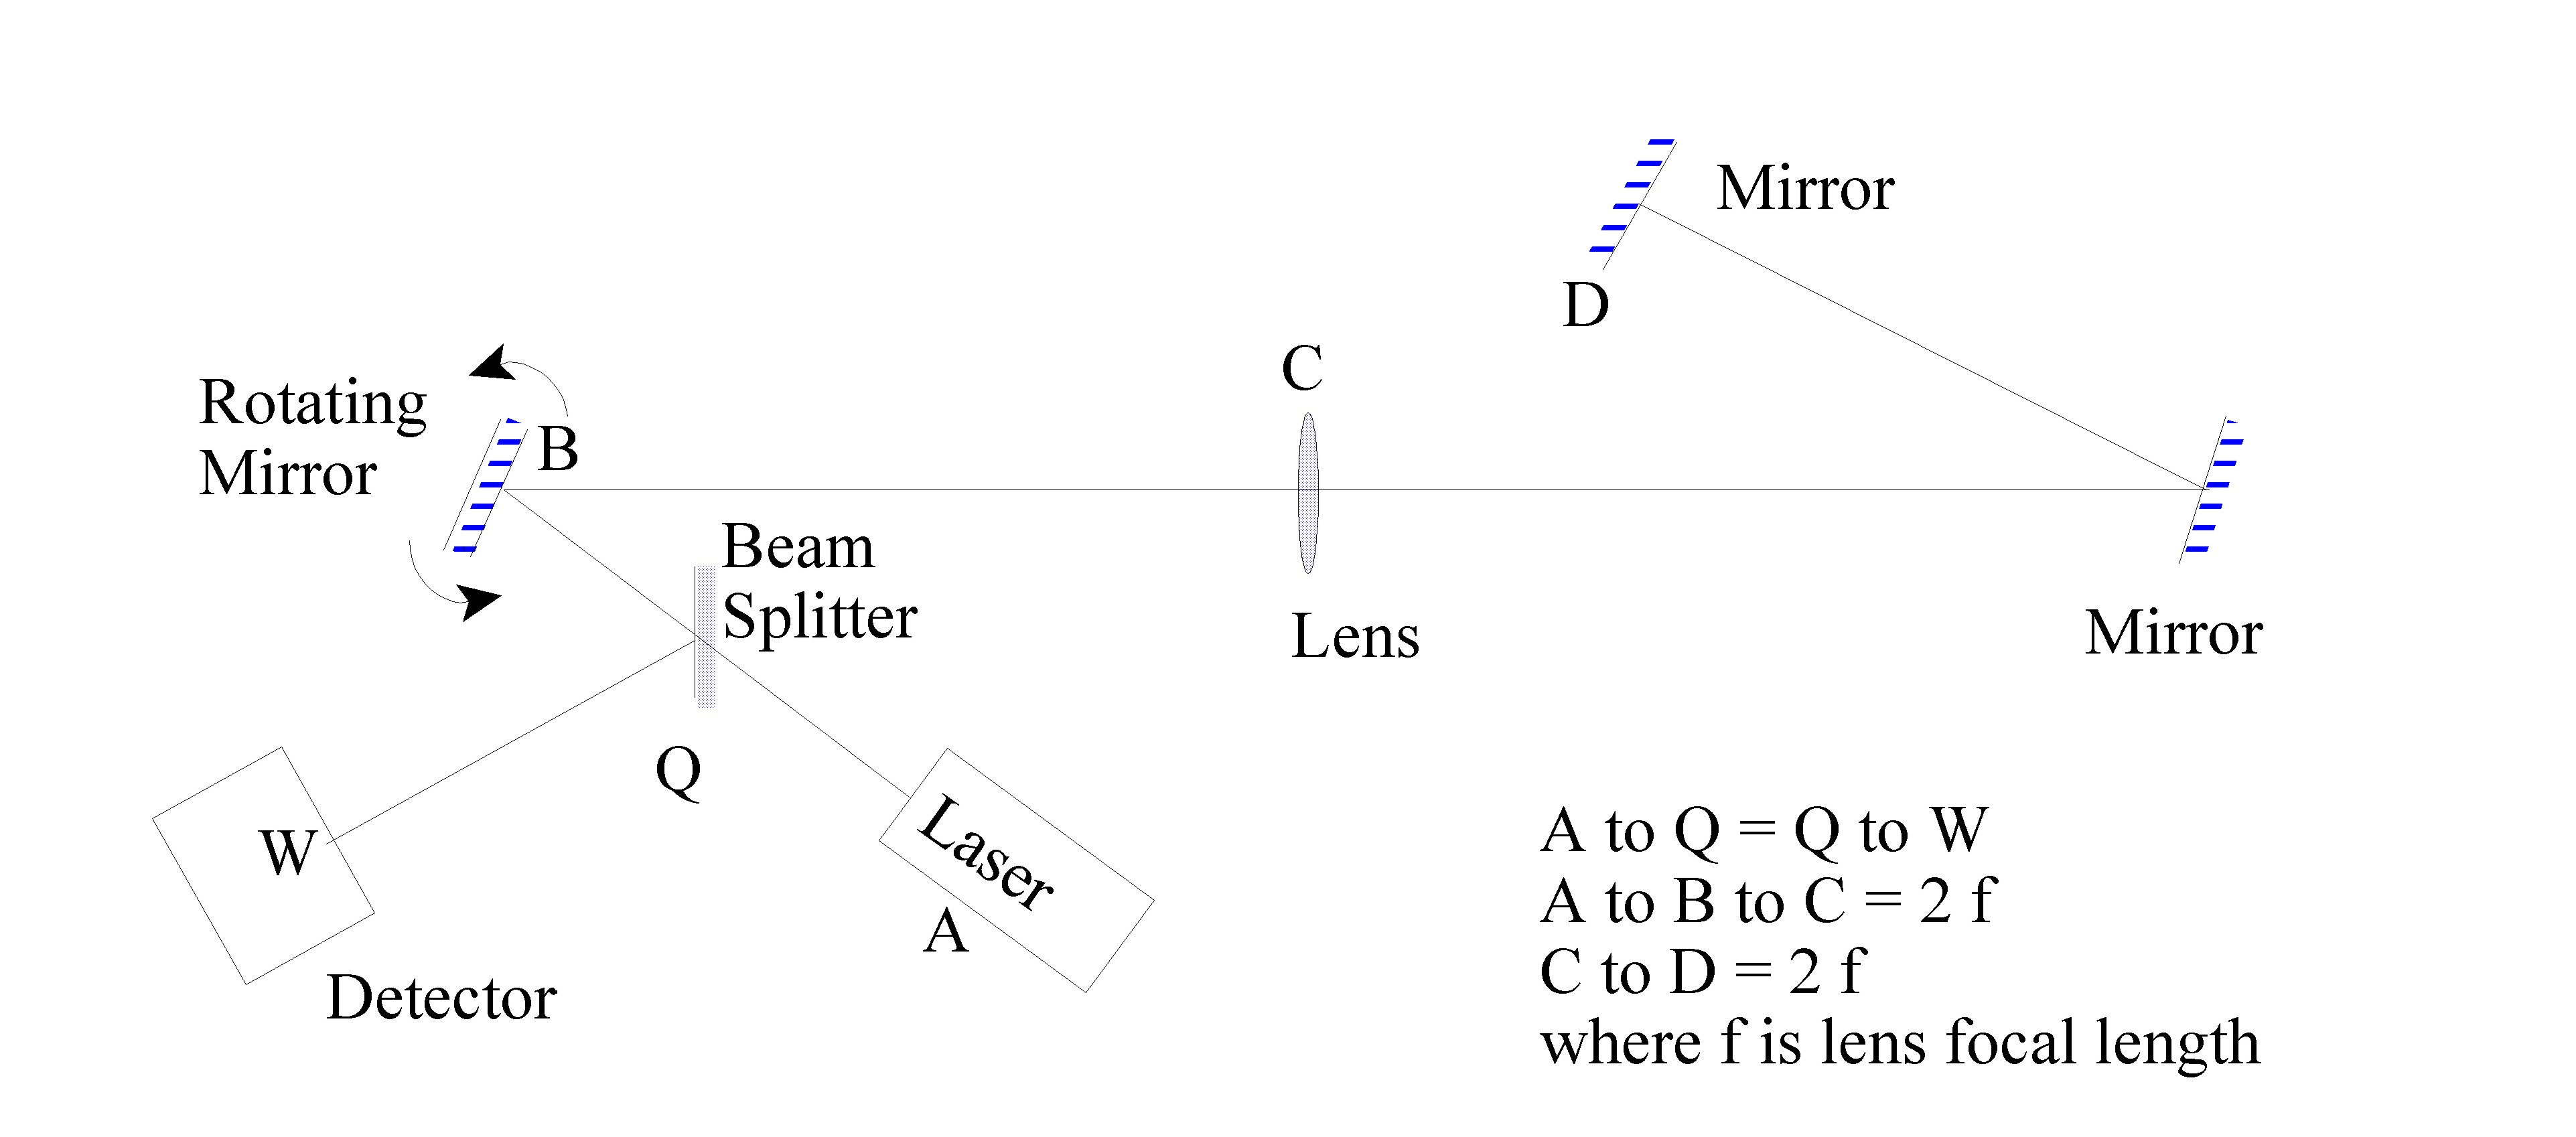
\includegraphics[width=230px]{Canvas/Diagram.jpg}
\caption{This figure is an example schematic of the Rotating Mirror experiment. The focal length of the lens used at point C is $4.75m$, meaning lengths WQBC, ABC, and CD are all $9.5m$. One important difference between this schematic and our experiment is that there is not mirror placed between the lens at C and the mirror at D, as we had enough room to make this a straight shot. This is only semantic though because this difference changes nothing about the experiment.}
\label{schematic}
\end{figure}

% Describe system 
At the heart of this experiment is the the schematic of the components used in this experiment, pictured in Figure \ref{schematic}.
One important difference between this schematic and the arrangement used in our experiment is that ours did not used the unlabeled mirror on the far right of Figure \ref{schematic} because we used an large room.
Ours was a straight shot from the lens at point C and the mirror at D.
Removing this mirror from the setup did not change anything about the theory of this experiment because all that matters is that the distance $CD=2f$, where $CD$ is the distance between points C and D and $f$ is the focal length of the lens. 

The most important value to know for the setup of this experiment is the focal length of the lens. 
This value directly controls the distances between the other parts in this schematic because we need the beam to be properly focused when it lands on the detector. 
The focal length of the lens we used was $4.75m$. 
The lengths of ABC, WQBC, and CD were all set to a value of $2f$ because at this value the beam would stay focused throughout the entire setup. 
Since WQBC and ABC are the same length and both include CBQ in their overall path length, WQ and AQ also were set to the same distance to create an easily resolvable dot. 

% rotating mirror
To run the rotating mirror we used the  Leybold Speed-of-Light kit and connected it to a Variac, a variable AC power supply.
With the rotating mirror and Variac connected, we could turn the knob on the Variac from 20\% to 90\% of the 120 volts from the wall to cause the rotating mirror to turn at different angular velocities. 
Using this configuration we got rotational frequencies of 115Hz to 515Hz. 

% detector
The detector plate, shown at point W on Figure \ref{schematic}, was constructed so that a Vernier caliper was taped parallel to the axis the dot would travel as the rotational frequency increased.
This gave an accurate and precise way to read the location of the light beam as it traveled along its path. 

% photodetector
Another necessary component was a photodetector, that was placed in the arc of the light beam after reflected off the mirror. 
It was important to place the photodetector close enough to the rotating mirror so the light intensity peaks would be discernible from noise. 
We placed it on the stand that was supporting the lens because of this.
Wires were then ran from the photodetector to an oscilloscope so the frequency at which the light beam hit the photodetector could be known.
The oscilloscope then read the frequency that the light passed over it, giving the rotational frequency of the rotating mirror. 

% Describe taking data
After setting up the experiment, as depicted in Figure \ref{schematic} without the mirror on the far right, we could begin to collect data. 
One person would change the voltage given to the rotating mirror and record the rotational frequency given by the oscilloscope.
The other person would watch the detector and record the values of the position of the light beam as it landed on it. 
To record the position values we took pictures of each dot location so the exact location of the dot could be found by zooming into the photo.


\section{Data Analysis}
% Explain the Results 
After collecting the data for this experiment, we were left with three sets of data.
One set was for the location that the light beam landed on the caliper, the next was the rotational frequency of the rotating mirror, and the last was the percentage of power we gave to the rotating mirror using the Variac.
Since the Variac was connected to a US wall outlet of 120V, we converted the percentage power value to the supplied voltage by multiplying the percentage by 120V.
Another value we have to analyze was the frequency that the oscilloscope was reading!
The value it gave was two times the actual frequency because the rotating mirror was double sided, meaning it was measuring twice every rotation, doubling the perceived frequency!
We simply divided those numbers by two to get the actual frequency of rotation. 
These initial data sets are listed in Table \ref{initial}.

\begin{figure}
\begin{tabular}{|c|c|c|}
\hline
Dot Distance [mm] & Frequency [Hz] & Voltage Supplied [V] \\
\hline
5.69	0(46)	&115(8)	&24.0(1)\\
5.470(46)	&210(8)	&32.4(1)\\
5.200(46)	&286(8)	&48.0(1)\\
4.920(46)	&342(8)	&60.0(1)\\
4.700(46)	&394(8)	&74.4(1)\\
4.570(46)	&432(8)	&84.0(1)\\
4.500(46)	&467(8)	&96.0(1)\\
4.340(46)	&515(8)&108.0(1)\\
\hline
\end{tabular}
\caption{This table shows the data for dot distance on the detector [mm], rotational frequency of the mirror [Hz], and the voltage supplied to the rotational mirror. The uncertainties of the dot distance and frequency were found from fitting the chi squared minimization of the rotational frequency and dot distance and the voltage and rotational frequency data respectively. The uncertainties in the voltage supplied data is a flat $0.1V$ based on us being a little off of the mark when going up by 10\%.  }
\label{initial}
\end{figure}

The goal of our data analysis was to find the relationship between the frequency and the displacement of the light beam;
however, before we could analyze those two data sets, we needed to look at the relationship between voltage and frequency to obtain uncertainties in the frequency that we will use in the final chi-squared minimization. 
We preformed a Chi-sqaured minimization on the voltage versus frequency data to yield the epsilon matrix for this data, which has the uncertainty information encoded in it.
Using the information stored in the epsilon matrix and our voltages, we found the uncertainties related to frequency depending on the voltage the rotating mirror was spun at, shown in Table \ref{sigmax}.

\begin{figure}
\begin{tabular}{|c|c|}
\hline
Voltage [V] & Sigma x \\
\hline
32.4	&6.3956\\
48.0	&4.7228\\
60.0	&3.7737\\
74.4	&3.4247\\
84.0	&3.7942\\
96.0	&4.7556\\
108	&6.0219\\
\hline
\end{tabular}
\caption{This table shows the uncertainty values found from preforming the chi squared minimization on the data from the rotational frequency and voltage supplied to the rotating mirror. The uncertainties in the epsilon matrix where manipulated and multiplied by the voltage to give uncertainties.}
\label{sigmax}
\end{figure}

After obtaining those values, we were able to preform the chi-square minimization between frequency and displacement.
The data used in this analysis and the fit given from it is shown in Figure \ref{finalchi} and Figure \ref{finalgraph}.
The displacement was found by taking our dot distance data, in Figure \ref{initial}, and subtracting every individual value by the first value to set every point in reference to it! 
Because we used the first point as calibration, it is excluded from the final minimization.

\begin{figure}
\begin{tabular}{|c|c|}
\hline
Slope & y-intercept \\
\hline
$3.7969(1767)\times 10^{-6}m/Hz$ & $-0.000556748(69087)m$\\
\hline
\end{tabular}
\caption{This table shows the slope and y-intercept of the chi squared minimization of the displacement vs frequency data! The uncertainties of these values were found by taking the square root of the values from the epsilon matrix. This fit was used to draw the trend line in figure \ref{finalgraph}.}
\label{finalchi}
\end{figure}

\begin{figure}
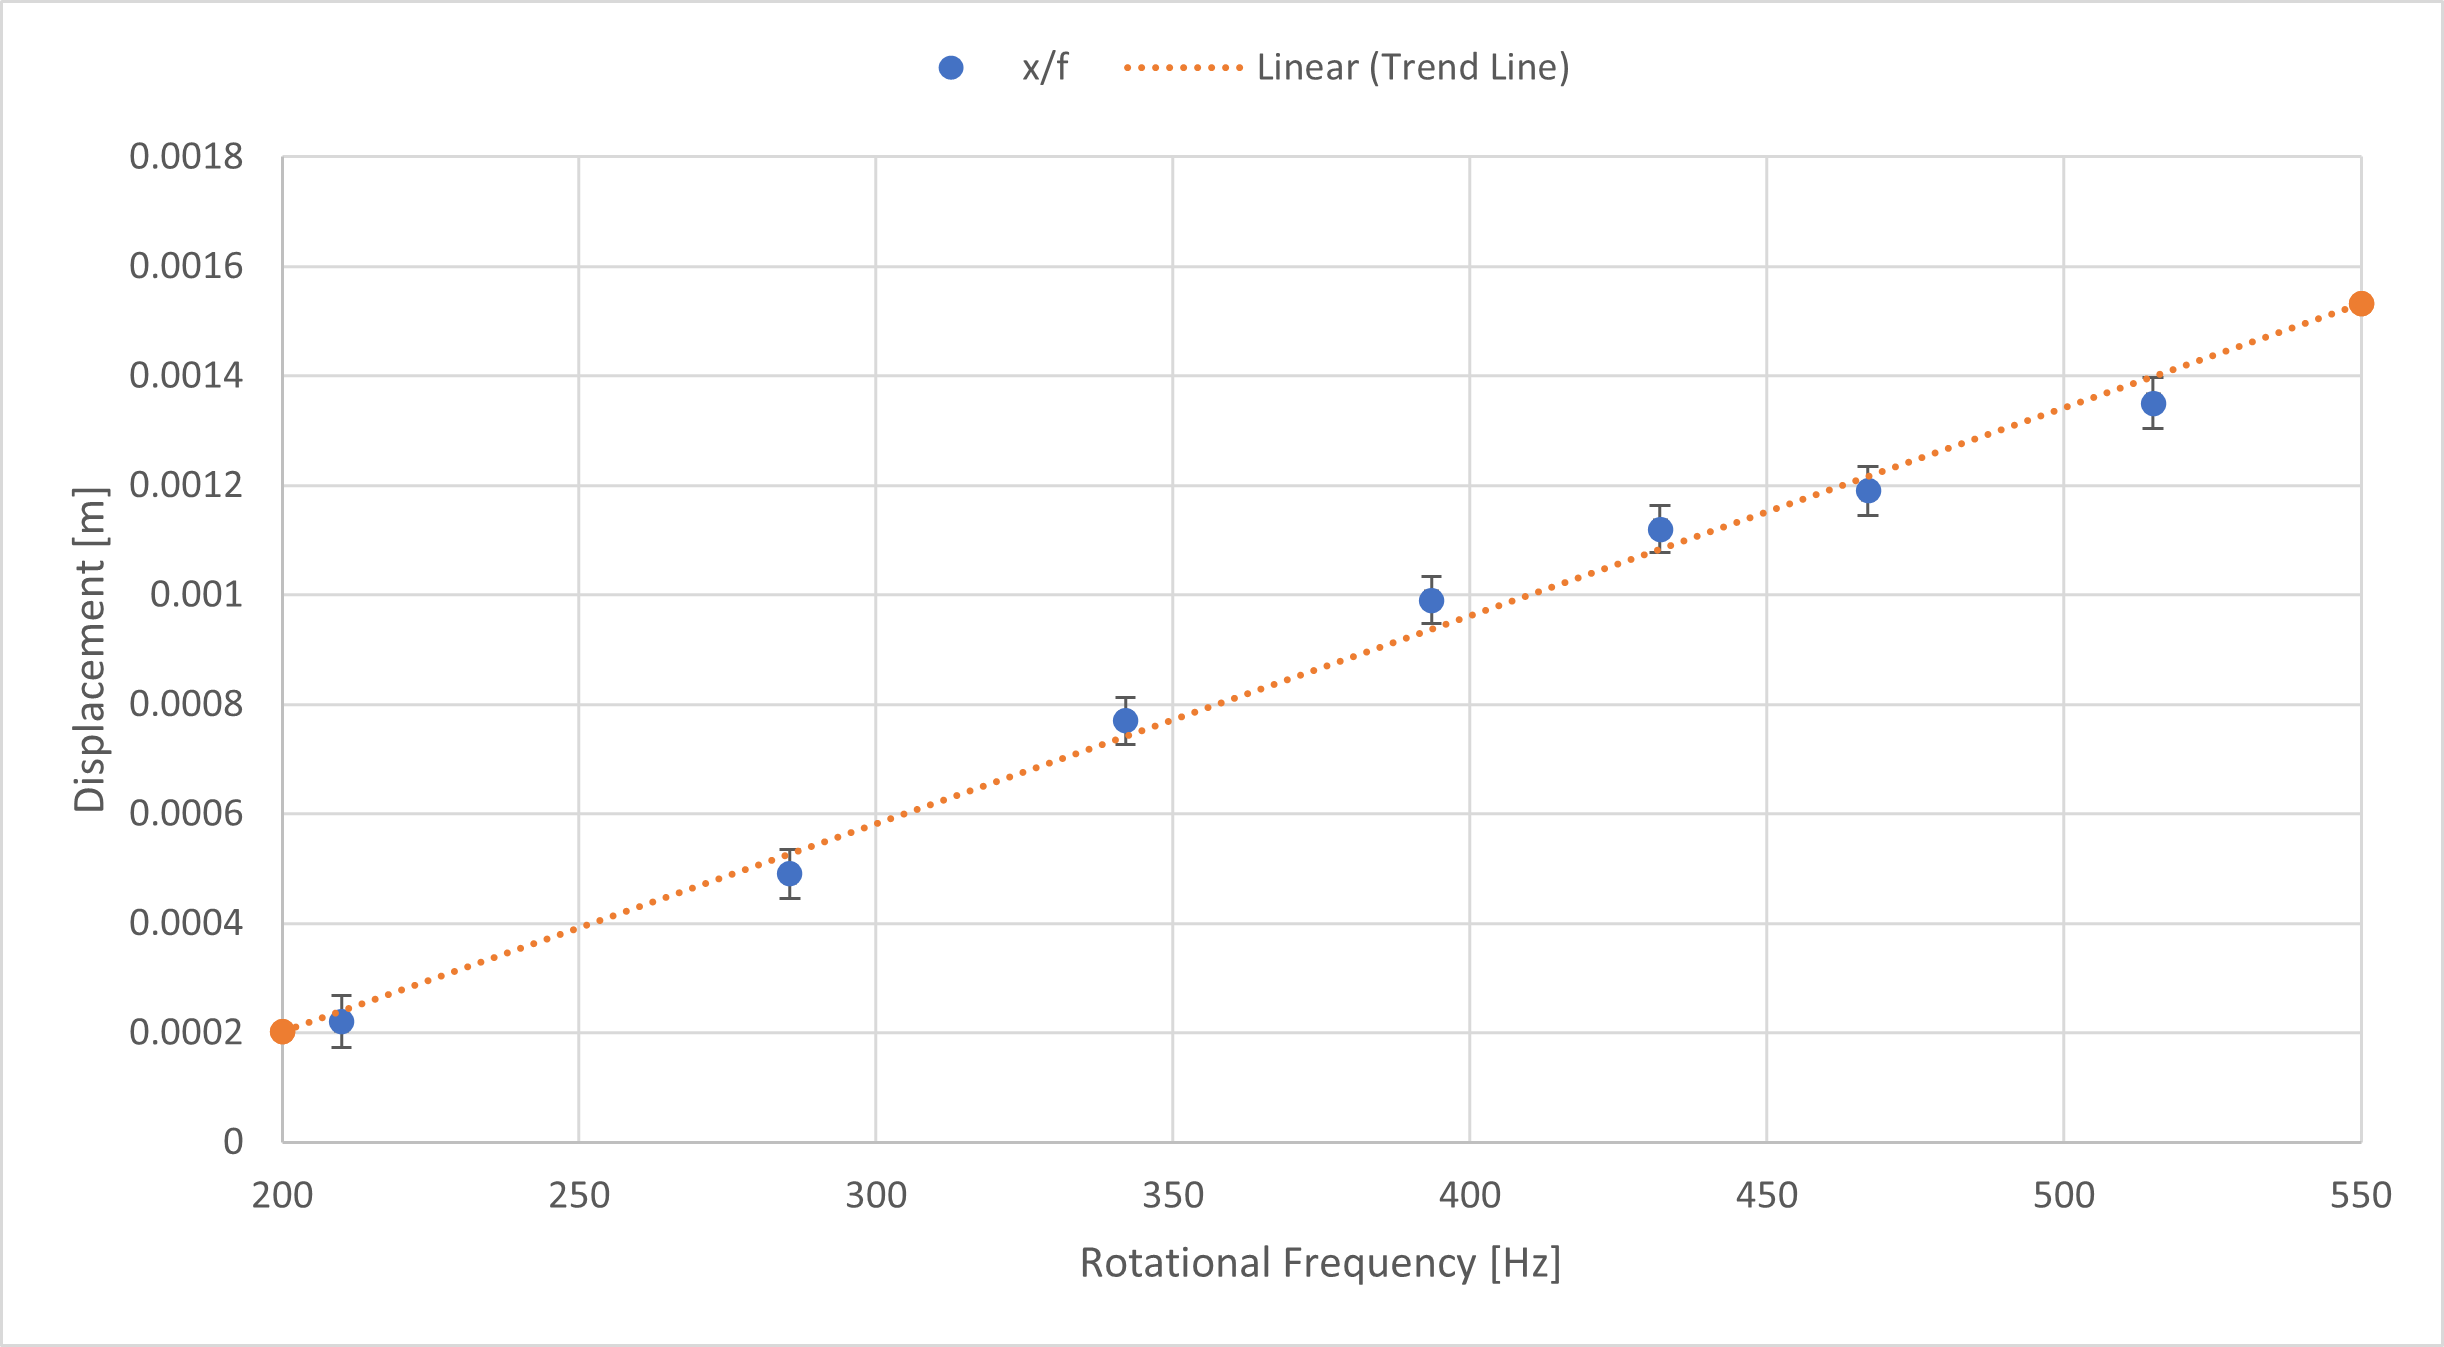
\includegraphics[width=230px]{finalgraph.png}
\caption{This figure shows the plot of our displacement versus rotational frequency data, with the trend line drawn from the data in table \ref{finalchi}. The solid blue dots represent the data points and the dotted orange line represents the linear regression preformed on those points. The error bars show the relative error of each data point and are the sigma values in the chi squared minimization.}
\label{finalgraph}
\end{figure}

From our final chi squared minimization we obtain a slope fit of $3.797(177)\times 10^{-6}\frac{m}{Hz}$. 
This is our $\frac{\delta x}{f}$ value.
If we look back at our equation \ref{answer}, we see we now know $l$ and $\frac{f}{\delta x}$.
Plugging into our equation we get $2.987(35)\times 10^{8}m/s^2$.

\section{Conclusion}
% Conclusion 
The accepted value of the speed of light is $299792458m/s^2$ \cite{NIST};
note that there is no uncertainty related with this value.
This is because the meter is defined based on some fraction of the speed of light;
therefore we have set the speed of light to be exactly equal to that, and everything else is based relative to this measurement. 
Our measured value of $2.987(35)\times 10^{8}m/s^2$ is within $2\sigma$ of the value of the speed of light!

The main improvement that could be made to this experiment is the method of recording the displacement!
We simply taped a caliper to the board to record the data.
This gave more precision than our attempts using a pen or pencil, but a very fine ruler would be even better!
The ruler on the side of the caliper went down to $0.25mm$ increments, which led to the uncertainty of the actual value to be high.

Another improvement is the focus and spread of the laser beam.
We made the beam as focused as we could get it on the detector board but it was still $30mm$ wide in some cases.
It was hard to decipher what exact point we should measure the laser being at, especially when the dot was not of a uniform radius.
This could be improved by using a laser with a smaller spread or by using another lens to focus the light more!

\begin{thebibliography}{9}
\bibitem{light} \textit{The Speed of Light}, Las Cumbres Observatory. (May 4, 2022). \url{https://lco.global/spacebook/light/speed-light/#:~:text=Galileo\%20concluded\%20that\%20the\%20speed,one\%20person\%20to\%20the\%20other.}.
\bibitem{engineer} C. McFadden, \textit{Physics in a Nutshell: A Brief History of the Speed of Light}, Interesting Engineering. (Apr 25, 2017). \url{https://interestingengineering.com/a-brief-history-of-the-speed-of-light}.
\bibitem{NIST} \textit{speed of light in vacuum} (National Institute of Standards and Technology, May 4, 2022).


\end{thebibliography}

\end{document}
